\documentclass[12pt, a4paper, spanish]{article}
\usepackage{amssymb}
\usepackage{amsmath}
\usepackage[a4paper=true]{hyperref}

\usepackage[top=4cm,bottom=2cm,left=2cm,right=2cm]{geometry}



%\usepackage[amsfonts]
\usepackage[spanish]{babel}
\usepackage[utf8]{inputenc}
\usepackage{packages/caratula}
\usepackage{packages/algo2symb}
\usepackage{packages/newalgo}
\usepackage{packages/itef}
\usepackage{graphicx}
\usepackage[T1]{fontenc}
\usepackage{makeidx}
\usepackage{listings}
\usepackage{color}

\usepackage{fancyhdr}
\usepackage{lastpage}
\pagestyle{fancy}

%matrices
\newcommand{\mW}{\ensuremath{{\bf W}}}
\newcommand{\mA}{\ensuremath{{\bf A}}}
\newcommand{\mD}{\ensuremath{{\bf D}}}
\newcommand{\mI}{\ensuremath{{\bf I}}}
\newcommand{\vx}{\ensuremath{{\bf x}}}
\newcommand{\ve}{\ensuremath{{\bf e}}}
\newcommand{\vz}{\ensuremath{{\bf z}}}

\newcommand{\norma}[1]{\left|\left|#1\right|\right|}
\newcommand{\tc}{\hbox{\bf tc}}
\newcommand{\real}{\ensuremath{\mathbb{R}}}
\newcommand{\nat}{\ensuremath{\mathbb{N}}}

\parskip=1ex
\pagestyle{fancy}
\fancyhf{}
\renewcommand{\headrulewidth}{0.02 cm}
\renewcommand{\footrulewidth}{0 cm}
\fancyhead[L]{Métodos Numéricos - Ranking de Page (¿y Plant?)}
\fancyhead[R]{Camino, Escalante, Giudici}
\fancyfoot[C]{\thepage}
\def\septad{\rule{16 cm}{.2 mm}}

\begin{document}
%
    \materia{Métodos Numéricos}
%
    \titulo{Trabajo Práctico 2: Ranking de Page (¿y Plant?)}
%
    \integrante{Ramiro Daniel Camino}{264/06}{ramirocamino@gmail.com}
%
    \integrante{José Luis Escalante Catacora}{822/06}{joe.escalante@gmail.com}
%
    \integrante{Juan Carlos Giudici}{827/06}{elchudi@gmail.com}
%
    \maketitle
    \tableofcontents
    \newpage

    \section{Abstract}

{\bf Palabras clave:}
\begin{itemize} 
    \item
    \item
    \item
    \item
\end{itemize}

    \newpage
    \section{Introducción Teórica}

\subsection{PageRank}

PageRank es un algoritmo que modela un proceso aleatorio de navegación a través de
distintas páginas Web, cuyo objetivo es generar un ranking de importancia de páginas,
que en la práctica se utiliza para refinar los resultados de búsquedas de texto en las mismas
para refinar los resultados por relevancia.\\

El problema se define como encontrar el autovector asociado al autovalor 1 de la matriz de transiciones
correspondientes a un grafo de páginas Web interconectadas. Dado que esta matriz se puede ajustar
para que sea estocástica, el autovector corresponde a la proporción de tiempo que pasa un navegante
aleatorio en una página, que en la realidad resulta un buen indicador de importancia.\\

La manera en cómo se modela el problema del ranking es usando una matriz de adyacencias.
Sea $W \in \mathbb{R}^{n \times n}$ donde $n$ es la cantidad de sitios indexados, luego el elemento
$w_{ij}$ es igual $1$ si existe un link de la página $i$ a la página $j$ y $0$ en caso
contrario. A su vez los links autoreferenciados se ignoran por lo que en diagonal tenemos todos valores nulos.\\

Ahora con $W$ podemos extraer la cantidad de links salientes de cada página,
simplemente sumando los elementos de la fila correspondiente. Llamamos $n_j$
al grado de la página $j$ donde $n_j = \sum^{n}_{i = 1} w_{ij}$.

\subsection{Matriz de transiciones}

Con la matriz de adyacencias originales, ahora queremos tomar sus datos y generar con ellos
una matriz estocástica que defina la probabilidad de clickear en un link al azar
en una página y transicionar hacia otra.\\

Para ello, consideramos $P$ la matriz que se obtiene a partir de tomar la matriz de
adyacecias y normalizando sus filas para que tengan norma 2 igual a 1. Es decir,
si una página tiene 2 links salientes, la probabilidad de clickear en uno de ellos
es $\frac{1}{2}$, con tres links es $\frac{1}{3}$, y así sucesivamente.\\

El problema que hay con esto es que no todas las páginas necesariamente tienen links
salientes, por lo que se asume que si un navegante llega a una página sin \textit{outlinks},
elige una página al azar sobre el universo de todas las páginas.\\

Para modelar esto, sea $\vec{d}$ un vector con longitud $n$, la posición $d_i$ toma los valores\\

\begin{math}
d_i =
\left\{
\begin{array}{ll}
0   & \mbox{si el sitio tiene links salientes}\\
1   & \mbox{si el sitio no tiene links salientes}
\end{array}
\right.
\end{math}\\

Luego, sea $\vec{v}$ un vector con logitud $v$ con $v_i = [\frac{1}{n}]$, definimos
la matriz $D$ como\\

\begin{math}
D = d^t * v
\end{math}\\

Luego definimos $P' = P + D$, que es estocástica.

\subsection{Teleporteo}

Además del manejo de navegación aleatoria, \textit{PageRank} considera una probabilidad de que
en cualquier momento el navegador eliga saltar a una nueva página al azar, sin considerar
los links de la página actual. Esto se llama \textit{teleporteo}, y se modela como un factor
$c$ que multiplica a $P'$  y una matriz $E \in R^{nxn}$, con una probabilidad uniforme de $\frac{1}{n}$.\\

Luego la expresión que resuelve el problema de \textit{PageRank} de la matriz de transiciones
con teleporteo, dado el vector de probabilidades $\vec{x}$, es\\

\begin{align*}
Ax & =(cP' + (1-c)E)^{t} \vec{x}
\end{align*}

\subsection{Resolución de PageRank}

La resolución de \textit{PageRank}, en su forma más básica, consiste en obtener el autovector
asociado al autovalor 1. La forma más simple de hacerlo es por medio del método de potencias
que funciona computando $A\vec{x}$ iterativamente hasta cumplir con un criterio de detención.\\

Este método presenta un problema práctico, en que la matriz de transiciones suele ser muy
esparsa, pero si se considera la información agregada por las matrices $E$ y $D$, la misma
resulta densa. A continuación veremos que esto se puede resolver.

\subsection{Cálculo alternativo de $x^{(k + 1)} = P_2x^{(k)}$}

Veamos primero cómo utilizando el algoritmo de Kamvar podemos optimizar el espacio requerido
en memoria para el almacenamiento de la matriz $P_2$ y el tiempo de ejecución requerido para ha
cer la multiplicación entre matrices y vectores.\\

\newcommand{\vectornorm}[1]{\left\|#1\right\|}
Queremos ver que el algoritmo propuesto por \cite[Algoritmo 1]{Kamvar2003} es equivalente
a la operación $\vec{y} = A\vec{x}$, para $A=(cP + (1-c)E)^{t}$, donde $P$ es la matriz
de transiciones de links, no ajustada por las páginas sin outlinks,
y $E$ es la matriz uniforme de teletransportación con valor $\frac{1}{n}$ en cada celda.\\

Para ello, expandimos las ecuaciones de ambos y veremos que las mismas producen el mismo cálculo.\\

Primero, la ecuación $A\vec{x}$ se desarrolla como\\
\begin{align*}
(c(P + D) + (1 - c)E)^{t} \vec{x}
\end{align*}

Y la matrix de \cite[Algoritmo 1]{Kamvar 2003} como
\begin{align*}
cP^{t}\vec{x} + (\vectornorm{\vec{x}}_1 - \vectornorm{\vec{y}}_1)\vec{v}
\end{align*}

donde $\vec{y}$ es el vector resultante de $cP^{t}\vec{x}$ y $\vec{v}$ es el vector de probabilidad
uniforme de valor $\frac{1}{n}$ en cada elemento. Luego planteamos la equivalencia

\begin{align*}
c(P + D)^{t} + (1-c)E^{t} \vec{x} &= cP^{t}\vec{x} + (\vectornorm{\vec{x}}_1 - \vectornorm{\vec{y}}_1)\vec{v} \\
cP^{t}\vec{x} + cD^{t}\vec{x} + (1-c)E^{t}\vec{x} &= cP^{t}\vec{x} + (\vectornorm{\vec{x}}_1 - \vectornorm{\vec{y}}_1)\vec{v} \\
cD^{t}\vec{x} + (1-c)E^{t}\vec{x} &= (\vectornorm{\vec{x}}_1 - \vectornorm{\vec{y}}_1)\vec{v}
\end{align*}

Veamos por qué el término del lado izquierdo es equivalente al derecho.\\

La norma 1 del vector es la suma de los valores absolutos de sus elementos.
Observemos que, para las columnas de $P$, las mismas o bien tienen norma 1 que vale 1, o cero.
Es decir, las columnas no-cero de $P$ contribuyen a la norma 1 de $\vec{y}$.\\

Observemos también que en la multiplicación $(1-c)E\vec{x}$, la norma 1 de este producto es
$(1-c)$, pues la norma 1 de cada columna de $E$ es 1 y $\vectornorm{\vec{x}} = 1$.\\

Por ultimo, también vemos que para aquellas columnas de ceros en $P^{t}$, las columnas no-cero de
 $D$ preservan la norma de las mismas.\\

Dados los hechos anteriores, podemos obervar que $\vectornorm{\vec{x}}_1 - \vectornorm{\vec{y}}_1$ se
puede interpretar como la norma que se ``pierde'' cuando $\vec{x}$  es multiplicada por $cP^t$.
Esta ``pérdida de norma'' se debe justamente a que falta sumar los products de $\vec{x}$  por
$E$  y $D$ de la ecuación, pues $A$ preserva la norma 1.\\

Ahora, como en $E^t$ y $D^t$, las filas que componen cada matriz son iguales entre sí (en $E^t$ todos elementos valen $\frac{1}{n}$, y
en $D^t$ como fue descrito en la sección anterior), cuando se realiza $E\vec{x}$ o $D^t\vec{x}$, el resultado
produce un vector de valores idénticos en cada posición. Estos mismos valores son la diferencia que captura
$(\vectornorm{\vec{x}}_1 - \vectornorm{\vec{y}}_1) \vec{v}$. Luego agregar esto a $\vec{y}$ resulta
equivalente a haber realizado las sumas de vectores resultantes correspondientes, con la diferencia
de que no hizo falta materializar dichas matrices.\\

Con ello concluimos que los dos términos del algoritmo de Kamvar son equivalentes
a la matriz $A$ de transiciones. $ \blacksquare $

\subsection{QR y Reflecciones de Householder}

Existen variadas formas de descomponer una matriz. En este trabajo en particular usaremos la descomposición $QR$,
la cual consiste en descomponer una matriz $A$ en una matriz ortogonal $Q$ y una triangular superior $R$
de manera que $A = QR$. Al tener descompuesta $A$ en esa forma y teniendo un sistema $Ax= b$,
la obtención del vector solución se realiza resolviendo el sistema $Rx = Q^{t}b$.\\

A su vez existen distintos procedimientos para poder hallar la descomposición $QR$ de una matriz.
Uno de ellos es las \textit{reflecciones de Householder}, procedimiento por el cual en cada iteración se obtienen ceros por debajo de la diagonal, llevando la matriz $A$ a ser la matriz $R$ diagonal superior.\\

\begin{center}
  \centering
  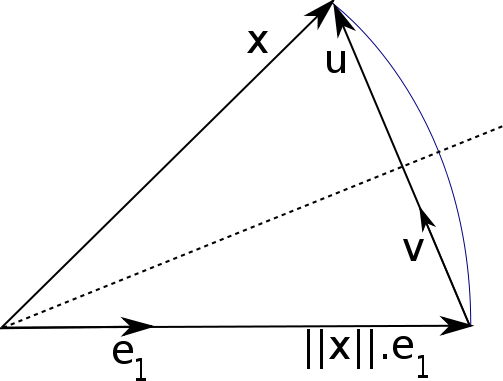
\includegraphics[scale=0.5]{./archivos/graficos/householder.png}
\end{center}

El objetivo es hallar una transformación lineal que cambie el vector $x$ en un vector de la misma longitud que sea colineal con $e_1$. Householder refleja a través de la línea punteada (elegida para dividir el ángulo entre $x$ y $e_1$). El máximo ángulo con esta transformación es a lo sumo de 45º.\\

Veamos un paso del procedimiento para poder ilustrar mejor: Sea $A \in \mathbb{R}^{n \times n}$ y sea $x_1$ el vector correspondiente a la primer columna de $A$ y $e_1$ el vector canónico, definimos:

\[
  \alpha_1 = \vectornorm{x_1}
\]
\[
  u = x_1 - \alpha_1 e_1
\]
\[
  v = \frac{u}{\vectornorm{u}}
\]
\[
  Q_1 = I - 2vv^{T}
\]

Luego $Q_1$ es la matriz que al multiplicarla a izquierda por $A$ coloca ceros por debajo de la diagonal.

\[
  Q_1A = \begin{bmatrix}
   \alpha_1&\star&\dots&\star\\
      0    &     &     &    \\
   \vdots  &     &  A' &    \\
      0    &     &     & \end{bmatrix}
\]

Repitiendo estos pasos: $Q_{n - 1} \dots Q_2Q_1A = R$. Luego el producto de las $Q$'s forma una matriz ortogonal, lo cual hace fácil y rápido hallar el vector solución del sistema.
\[
  Q^T = Q_{n - 1} \dots Q_2Q_1
\]
\[
  Ax = b \iff Q^TAx = Q^Tb \iff Rx = Q^Tb
\]


    \newpage
    \section{Desarrollo}
 % * Detalles de implementacion: Mencionar como se encaro el trabajo, la primera implementacion en python y la version final en C++. En python se uso scipy con matrices esparsas y optimizamos el codigo y todo corre rapido para los datasets mas grandes que encontramos
 % * en C se decidio utilziar STL y map<map<>> para la matriz esparsa, solo se implementaron las operaciones necesarias para correr el agoritmo
 % * dependiendo el algoritmo y x0 no es necesario normalizar al final
 % * probar con un dataset grande -- no pudimos porque quedaron mas grandes los que bajamos (alto chamuyo!!! weeeeeoonnn)
 % * para hacer QR decidimos hacer todos los pasos a mano (sin iteraciones) ya que son solo dos, porque es una matrix de 2x2, cita al paper con resolucion linda Gram-Schmidt (Algorithm 7)
 % * se decidio utilizar como criterio de parada la chingada diferencia de norma1 por la mismas razones que kamvar (citar el paper y hacer mini mini resumen)

\subsection{Detalles de Implementación} % (fold)
\label{sub:detalles_de_implementaci_n}

\subsubsection{Enfoque Inicial - Etapa Python} % (fold)
\label{ssub:enfoque_inicial}

En principio para evitarnos detalles de manejo de memoria y contar con una mayor
de expresividad de lenguaje, implementamos el trabajo en Python.

Usando librerías como Numpy y Scipy, pudimos hacer uso de matrices
esparsas y operarlas cómodamente de manera eficiente; dado
que las distintas clases de matrices esparsas disponibles
exponen la misma interfaz, pudimos probar entre varias hasta encontrar
una que funcione para nuestro caso de uso.

Tan sólo unas horas de trabajo y terminamos una implementación
que devolvía resultados que parecían correctos. Inclusive con datasets
enormes, como los que se pueden encontrar en la página de Stanford,
el programa en Python tardaba pocos segundos por iteración y en cuestión de minutos armaba el ranking.

Las únicas diferencias sustanciales de tiempo aparecían en la lectura del archivo de entrada
y armado de la matriz inicial, donde el overhead en Python dominaba y no había
ningún conjunto de subrutinas optimizadas para esa tarea.

\subsubsection{Implementación - Etapa C++} % (fold)
\label{ssub:implementaci_n_etapa_c_}

Una vez habiendo comprobado que la idea de cómo implementar este trabajo
funcionaba, es que usamos el código de Python a manera de pseudocódigo para el de C++.

En C++ para armar las matrices esparsas usamos STL y la estructura de datos
\textit{std::map}, que expone una interfaz de contenedor genérico que preserva órden, internamente
implementado como un Red-Black tree.

A diferencia de la implementación en Python donde hacemos uso indiscriminado
de la riqueza de las librerías, nos vimos forzados a acomodar las operaciones
de manera tal que tengamos que implementar solamente las operaciones exclusivamente necesarias.

La reclamación de recursos de memoria es uno de los mayores problemas de usar
lenguajes con manejo de memoria manual. Esto en la práctica no resultó ser un problema,
dado que tomamos ventaja de las faciliades de manejo de memoria provistas por la nueva versión
de C++: los \textit{unique\_ptr} y los \textit{shared\_ptr}, que permiten reclamar objetos que se van fuera de
\textit{scope}, y en el caso de los \textit{unique\_ptr}, también garantizan que un objeto tenga
una sola variable como ``dueño'' a la vez, permitiendo razonar más facilmente sobre la misma.

Un problema que sí hubo, fue que nuestro primer intento de implementación intentaba simplificar
las operaciones matriciales haciendo uso de la sobrecarga de operadores en C++. El problema
con esto es que los operadores retornan objetos por copia, por lo que cada operación numérica
hecha con estos implicaría una copia masiva de datos (en teoria C++ soporta una clase de optimización
llamada \textit{elisión de copia} para evitar retornar objetos por copia, pero su utilización es muy acotada y
es difícil contar con la misma siempre).

Para resolver esto, implementamos las operaciones con variantes que pasan objetos por referencia, y
en muchos casos, para ahorrar memoria, hicimos operaciones que modifican la matriz original. En la práctica
esto fue necesario, dado que varias matrices esparsas llegaban a consumir múltiples gigabytes de memoria.
% subsubsection implementaci_n_etapa_c_ (end)


% subsubsection enfoque_inicial (end)

% subsection detalles_de_implementaci_n (end)

    \newpage
    \section{Resultados}

    \newpage
    \section{Discusión y Conclusiones}

\subsection{Convergencia del Método de la Potencia}

Como podemos ver en la Sección~\ref{sec:convergencia} la convergencia del
Método de la Potencia no depende de los nodos ni de los links (tamaño) del
grafo a analizar. En cambio como podemos ver en el Cuadro~\ref{tab:iteraciones}
sí depende del factor de teletransportación $c$ elegido. A mayor $c$ mayor son
las iteraciones necesarias para la convergencia.

\subsection{Beneficios de la Extrapolación Cuadrática}

Se puede ver claramente en el Cuadro~\ref{tab:iteraciones} los beneficios de
realizar Extrapolaciones Cuadráticas. El beneficio se encuentra en el rango del
$27\%$ al $44\%$.

Es muy interesante el comportamiento de la cantidad de iteraciones necesarias
en base a la frequencia de realizar iteraciones con Extrapolación Cuadrática.
El beneficio de incorporar estas iteraciones es claro, pero una frecuencia muy
alta perjudica su beneficio. Para todos los $c$ realizar una Extrapolación
Cuadrática cada 4 o 5 iteraciones se comporta peor que realizar una cada 10
iteraciones.

La Extrapolación Cuadrática para el Método de la Potencia es una aproximación
de una iteración imaginando esta como una combinación lineal de los primeros
tres autovectores. El paper de KamvarREFFF muestra empíricamente sin ningún
sustento teórico que esta aproximación es mejor que realizar la siguiente
iteración del Método de la Potencia.

En nuestro caso, al aplicar esta aproximación muy seguido, sin dejar que el
Método de la Potencia mejore por si sólo, el resultado nos produce menor
beneficio. Nuestra hipótesis es que se debe a que al utilizar sólo tres
autovectores para la aproximación se pierde la influencia de los siguientes
autovectores que parece no ser menor. Por esto, necesita de varias iteraciones
del Método de la Potencia para que la aproximación vuelva a traer grandes
beneficios.

Por último no calculamos el tiempo que influye realizar una iteración con
Extrapolación Cuadrática, pero en KamvarREFFF se postula que es despreciable en
comparación con el beneficio otorgado.

\subsection{Trabajo futuro}

Proponemos el siguiente trabajo futuro basado en los resultados, conclusiones y
experiencias obtenidas a lo largo del desarrollo de este trabajo:

\begin{itemize}

\item Medir el tiempo necesario para agregar una Extrapolación Cuadrática. No
creemos que el beneficio práctico temporal sea muy diferente que el beneficio
de convergencia en cantidad de iteraciones, como esta postulado en KamvarREFFF.
No obstante se podría validar experimentalmente.

\item Analizar detalladamente la frecuencia óptima para realizar iteraciones
con Extrapolaciones Cuadráticas. En nuestro caso encontramos que realizar una
iteración con Extrapolación Cuadrática cada 10 iteraciones es mejor que cada 4
o 5 iteraciones, pero es probable que sea otra la frecuencia óptima. También
puede darse el caso donde dejar ``descansar'' al algoritmo durante varias
iteraciones sin realizar Extrapolación Cuadrática y luego realizarla nuevamente
frecuentemente mejore a los resultados.

\item Analizar el comportamiento con otras instancias de prueba y comparar
entre sí. La instancia que utilizamos para las pruebas es real, pero acotada.
Los resultados pueden llegar a variar según diferentes datasets, dependiendo
cuán importantes son los autovectores siguientes al tercero (según nuestra
hipótesis).

\item Calcular más autovalores y sus autovectores asociados para ver si la
hipótesis previa donde postulamos que estos tienen mucha influencia en cada
iteracion tiene fundamento o carece de él.

\end{itemize}

    \newpage
    \section{Conclusiones}

\subsection{Matriz Rala}

Dado los resultados obtenidos en ambos algoritmos, nuestra implementación de la matriz rala nos resulto mal encaminada, la decisión de hacerla estática nos jugó en contra al momento de hacer la factorización QR con rotaciones de givens, ya que la matriz a factorizar se tiene que cambiar por cada 0 que se pone debajo de la diagonal, lo cual implica volver a crear la matriz por cada paso demorando el cálculo del mismo. 

De todas formas, nuestra algoritmo iterativo con respecto a la matriz rala, aumenta la capacidad de procesamiento en cuanto al tamaño del caso, pero perdiendo precisión en los cálculos.

\subsection{Método Iterativo}

El método iterativo se presenta como una alternativa a resolver los casos que el método directo no puede abordar gracias al tamaño del mismo, solamente tenemos que tener en cuenta que si queremos una mayor precisión tenemos que sacrificar tiempo, por lo tanto, si el tiempo no es problema, podemos hacer mas iteraciones obteniendo un mejor resultado. Como la velocidad de convergencia es relativamente rapida al principio, se pueden obtener buenos resultados con pocas iteraciones, logrando una un resultado aceptable relativamente rapido.

\subsection{Método Directo}

El método directo se vio directamente afectado por nuestra implementación de la matriz rala, como bien dijimos antes, nuestra implementación nos obligaba a reconstruir la matriz a factorizar por cada paso de la factorización QR. De todas formas en los casos en que pudimos correr el método, obtuvimos los resultados esperados y el algoritmo funciona correctamente. 

Este método es el ideal para casos chicos de prueba, o una vez mejorada en un futuro la matriz rala, poder abarcar casos mas grandes.
    \newpage

    \appendix
    \section{Enunciado}

\begin{center}
\begin{tabular}{r|cr}
 \begin{tabular}{c}
{\large\bf\textsf{\ M\'etodos Num\'ericos\ }}\\ 
Segundo Cuatrimestre 2013\\
{\bf Trabajo Pr\'actico 3}
\end{tabular} &
\begin{tabular}{l @{}}
 \emph{Departamento de Computaci\'on} \\
 \emph{Facultad de Ciencias Exactas y Naturales} \\
 \emph{Universidad de Buenos Aires} \\
\end{tabular} 
\end{tabular}
\end{center}

\vskip 25pt
\hrule
\vskip 11pt
 
\textbf{Introducci\'on}

A partir de la evoluci\'on de Internet durante la d\'ecada de 1990, el desarrollo de motores de b\'usqueda se ha convertido
en uno de los aspectos centrales para su efectiva utilizaci\'on. Hoy en d\'ia, sitios como Yahoo, Google y Bing ofrecen
distintas alternativas para realizar b\'usquedas complejas dentro de un red que contiene miles de millones de p\'aginas
web. 

En sus comienzos, una de las caracter\'isticas que distngui\'o a Google respecto de los motores de b\'usqueda de la \'epoca
fu\'e la calidad de los resultados obtenidos, mostrando al usuario p\'aginas relevantes a la
b\'usqueda realizada. El esquema general de los or\'igenes de este motor de b\'usqueda es brevemente explicando en 
Brin y Page \cite{Brin1998}, donde se mencionan aspectos t\'ecnicos que van desde la etapa de obtenci\'on de
informaci\'on de las p\'aginas disponibles en la red, su almacenamiento e indexado y su posterior procesamiento,
buscando ordenar cada p\'agina de acuerdo a su importancia relativa dentro de la red. El algoritmo utilizado para esta
\'ultima etapa es denominado PageRank y es uno (no el \'unico) de los criterios utilizados para ponderar la importancia
de los resultados de una b\'usqueda. En este trabajo nos concentraremos en el estudio y desarrollo del algoritmo
PageRank.

\textbf{El problema}

El algoritmo PageRank se basa en la construcci\'on del siguiente modelo. Supongamos que tenemos una red con $n$ p\'aginas 
web $Web = \{1,\dots,n\}$ donde
el objetivo es asignar a cada una de ellas un puntaje que determine la importancia relativa de la misma respecto de las
dem\'as. Para modelar las relaciones entre ellas, definimos la \emph{matriz de conectividad} $W \in \{0,1\}^{n \times n}$ 
de forma tal que $w_{ij} = 1$ si la p\'agina $j$ tiene un link a la p\'agina $i$, y $w_{ij} = 0$ en caso contrario. 
Adem\'as, ignoramos los \emph{autolinks}, es decir, links de una p\'agina a s\'i misma, definiendo $w_{ii} = 0$. Tomando 
esta matriz, definimos el grado de la p\'agina $j$, $n_j$, como la cantidad de links salientes hacia otras p\'aginas 
de la red, donde $n_j = \sum_{i = 1}^n w_{ij}$. Adem\'as, notamos con $x_j$ al puntaje asignado a la p\'agina $j\in
Web$, que es lo que buscamos calcular.

La importancia de una p\'agina puede ser modelada de diferentes formas. Un link de la p\'agina $u \in
Web$ a la p\'agina $v \in Web$ puede ser visto como que $v$ es una p\'agina importante. Sin embargo, no queremos que una
p\'agina obtenga mayor importancia simplemente porque es apuntada desde muchas p\'aginas. 
Una forma de limitar esto es ponderar los links utilizando la importancia de la p\'agina de origen. En otras palabras,
pocos links de p\'aginas importantes pueden valer m\'as que muchos links de p\'aginas poco importantes. En particular,
consideramos que la importancia de la p\'agina $v$ obtenida mediante el link de la p\'agina $u$ es proporcional a la 
importancia de la p\'agina $u$ e inversamente proporcional al grado de $u$. Si la p\'agina $u$ contiene $n_u$ links,
uno de los cuales apunta a la p\'agina $v$, entonces el aporte de ese link a la p\'agina $v$ ser\'a $x_u/n_u$. Luego,
sea $L_k \subseteq Web$ el conjunto de p\'aginas que tienen un link a la p\'agina $k$. Para cada p\'agina pedimos que
\begin{eqnarray}
x_k = \sum_{j \in L_k} \frac{x_j}{n_j},~~~~k = 1,\dots,n. \label{eq:basicmodel}
\end{eqnarray}
Definimos $P \in  \mathbb{R}^{n \times n}$ tal que $p_{ij} = 1/n_j$ si $w_{ij} = 1$, y $p_{ij} = 0$ en caso contrario. Luego,
el modelo planteado en (\ref{eq:basicmodel}) es equivalente a encontrar un $x\in \mathbb{R}^n$ tal que $Px = x$, es
decir, encontrar (suponiendo que existe) un autovector asociado al autovalor 1 de una matriz cuadrada, tal que $x_i \ge
0$ y $\sum_{i = 1}^n x_i = 1$. En
Bryan y Leise \cite{Bryan2006} y Kamvar et al. \cite[Secci\'on 1]{Kamvar2003} se analizan ciertas condiciones que debe
cumplir la red de p\'aginas para garantizar la existencia de este autovector.

Una interpretaci\'on equivalente para el problema es considerar al \emph{navegante aleatorio}. \'Este empieza en una
p\'agina cualquiera del conjunto, y luego en cada p\'agina $j$ que visita sigue navegando a trav\'es de sus links,
eligiendo el mismo con probabilidad $1/n_j$. Una situaci\'on particular se da cuando la p\'agina no tiene links salientes. En
ese caso, consideramos que el navegante aleatorio pasa a cualquiera de las p\'agina de la red con probabilidad $1/n$.
Para representar esta situaci\'on, definimos $v \in \mathbb{R}^{n \times n}$, con $v_i = 1/n$ y $d \in \{0,1\}^{n}$ donde 
$d_i = 1$ si $n_i = 0$, y $d_i = 0$ en caso contrario. La nueva matriz de transici\'on es 
\begin{eqnarray*}
D & = & v d^t \\
P_1 & = & P + D.
\end{eqnarray*}
Adem\'as, consideraremos el caso de que el navegante aleatorio, dado que se encuentra en la p\'agina $j$, decida visitar
una p\'agina cualquiera del conjunto, independientemente de si esta se encuentra o no referenciada por $j$ (fen\'omeno
conocido como \emph{teletransportaci\'on}). Para ello, consideramos que esta decisi\'on se toma con una probabilidad
$c \ge 0$, y podemos incluirlo al modelo de la siguiente forma:
\begin{eqnarray*}
E & = & v \bar{1}^t \\
P_2 & = & cP_1 + (1-c)E,
\end{eqnarray*}
\noindent donde $\bar{1} \in \mathbb{R}^n$ es un vector tal que todas sus componenetes valen 1. La matriz resultante
$P_2$ corresponde a un enriquecimiento del modelo formulado en (\ref{eq:basicmodel}). Probabil\'isticamente, la
componente $x_j$ del vector soluci\'on (normalizado) del sistema $P_2 x = x$ representa la proporci\'on del tiempo que,
en el largo plazo, el navegante aleatorio pasa en la p\'agina $j \in Web$.

En particular, $P_2$ corresponde a una
matriz \emph{estoc\'astica por columnas} que cumple las hip\'otesis planteadas en Bryan y Leise \cite{Bryan2006} y
Kamvar et al. \cite{Kamvar2003}, tal que $P_2$ tiene un autovector asociado al autovalor 1, los dem\'as autovalores de
la matriz cumplen $1 = \lambda_1 > |\lambda_2| \ge \dots \ge |\lambda_n|$ y, adem\'as, la dimensi\'on
del autoespacio asociado al autovalor $\lambda_1$ es 1. Luego, la soluci\'on al sistema $P_2 x = x$ puede ser calculada
de forma est\'andar utilizando el m\'etodo de la potencia.

\textbf{Enunciado}

El objetivo del trabajo es implementar el algoritmo PageRank, considerando dos m\'etodos distintos para el c\'alculo del
autovector principal de la matriz $P_2$. Para ello, se considera el entorno de aplicaci\'on real del algoritmo, donde el
n\'umero total de p\'aginas, $n$, es considerablemente grande (i.e., todas las p\'aginas web accesibles p\'ublicamente).
El programa tomar\'a como entrada un archivo con la representaci\'on de grafo de conectividad, construir\'a la matriz
$P_2$ definida en la secci\'on anterior y ejecutar\'a el algoritmo PageRank utilizando el m\'etodo de la potencia y una 
variante del mismo para distintas instancias de prueba. Se pide:

\begin{enumerate}
\item En base a su definici\'on, $P_2$ no es una matriz esparsa. Sin embargo, en Kamvar et al. \cite[Algoritmo
1]{Kamvar2003} se propone una forma alternativa para computar $x^{(k+1)} = P_2 x^{(k)}$. Mostrar que el c\'omputo
propuesto es equivalente. Utilizarlo para mejorar el espacio requerido en memoria para el almacenamiento de la matriz
$P_2$ y el tiempo de ejecuci\'on requerido para hacer la multiplicaci\'on entre matrices y vectores. 

\item Bas\'andose en el an\'alisis del punto anterior, implementar el m\'etodo de la potencia para calcular el
autovector principal de la matriz $P_2$.

\item Implementar la variante del M\'etodo de la Potencia propuesta en Kamvar et al. \cite[Secci\'on 5]{Kamvar2003},
denominada Extrapolaci\'on Cuadr\'atica. El m\'etodo de Cuadrados M\'inimos involucrado debe ser resuelto utilizando la
Factorizaci\'on QR de la matriz mediante alguno de los m\'etodos vistos en la materia.

\item Realizar experimentos considerando distintas instancias de prueba. Para ello, se podr\'a utilizar el c\'odigo
adjuntada para la generaci\'on de instancias en base a datos reales, o cualquier otra herramienta que el grupo considere
necesaria. Evaluar tambi\'en los algoritmos alguno de los conjuntos de instancias
provistos en \cite{SNAP}. Para cada algoritmo, analizar el tiempo de
ejecuci\'on, la evoluci\'on del error entre iteraciones consecutivas y considerar distintos criterios de parada. 
Adem\'as, analizar la calidad del ordenamiento obtenido en t\'erminos de la relevancia de las p\'aginas.
\end{enumerate}

\textbf{Formato de archivos}

El programa deber\'a recibir como par\'ametro un archivo con la representaci\'on esparsa de la matriz (grafo) de
conectividad. El archivo contendr\'a una l\'inea con la cantidad de p\'aginas ($n$), la cantidad de links ($m$) y luego
una lista con un link por l\'inea, indicando la p\'agina de origen y destino separadas por un espacio. A modo de
ejemplo, a continuaci\'on se muestra el archivo de entrada correspondiente al ejemplo propuesto en Bryan y Leise
\cite[Figura 1]{Bryan2006}: 

\begin{verbatim}
4 
8 
1   2
1   3
1   4
2   3
2   4
3   1
4   1
4   3
\end{verbatim}

Una vez ejecutado el algoritmo, el programa deber\'a generar un archivo de salida que contenga una l\'inea por cada
p\'agina, acompa\~nada del puntaje obtenido por el algoritmo PageRank, ordenados en forma decreciente en funci\'on de
este \'ultimo valor.

Para generar instancias, es posible utilizar el c\'odigo Python provisto por la c\'atedra. Es importante mencionar que, para que el mismo funcione, es
necesario tener acceso a Internet. En caso de encontrar un bug en el mismo, por favor contactar a los docentes de la
materia a trav\'es de la lista. Desde ya, el c\'odigo puede ser modificado por los respectivos grupos agregando todas
aquellas funcionalidades que consideren necesarias.

\vskip 15pt

\hrule

\vskip 11pt


{\bf \underline{Fechas de entrega}}
\begin{itemize}
 \item \emph{Formato Electr\'onico:} Domingo 10 de Noviembre de 2013, hasta las 23:59 hs, enviando el trabajo (informe +
 c\'odigo) a la direcci\'on \verb+metnum.lab@gmail.com+. El subject del email debe comenzar con el texto \verb+[TP3]+
 seguido de la lista de apellidos  de los integrantes del grupo.
 \item \emph{Formato f\'isico:} Lunes 11 de Noviembre de 2013, de 17 a 18 hs.
\end{itemize}

\noindent \textbf{Importante:} El horario es estricto. Los correos recibidos despu\'es de la hora indicada ser\'an considerados re-entrega.

\section{Referencias}

\begin{itemize}
    \item Numerical Analysis, Richard L. Burden, John Douglas Faires. Cengage Learning, 2005.
    \item The Linear Algebra behind Google, Bryan, Kurt and Leise, Tanya, SIAM Review, 2006.
    \item The anatomy of a large-scale hypertextual Web search engine, Brin, Sergey and Page, Lawrence, Computer Networks and ISDN Systems, 1998.
    \item Extrapolation methods for accelerating PageRank computations, Kamvar, Sepandar D. and Haveliwala, Taher H. and Manning, Christopher D. and Golub, Gene H., ACM, 2003.
\end{itemize}

    \newpage
    %\section{Referencias}
% Es importante incluir referencias a libros, articleculos y paginas de
% Internet consultados durante el desarrollo del trabajo, haciendo referencia a
% estos materiales a lo largo del informe. Se deben citar tambien las
% comunicaciones personales con otros grupos


\end{document}

